% ============================================================================
% RECONSTRUCTED from paper_ieee_access.pdf (text extraction), July 2026.
% This is NOT the authors' original lost .tex source. Content and structure
% follow the PDF; wording may differ slightly from the camera-ready file.
% Authors filled from the repository README (PDF had placeholder names).
% Figure files: fig1_frontier, fig2_protocol (= PDF Fig.~3 trap),
% fig3_provider_heatmap (= PDF Fig.~4), fig5_calibration (= PDF Fig.~5).
% PDF Fig.~2 (seed fix) is rendered as a code box.
% ============================================================================
\documentclass[journal]{IEEEtran}

\usepackage{amsmath,amssymb,amsfonts}
\usepackage{graphicx}
\usepackage{booktabs}
\usepackage{multirow}
\usepackage{cite}
\usepackage{url}
\usepackage{hyperref}
\usepackage{xcolor}
\usepackage{listings}

\graphicspath{{figures/}{../results/latest/figures/}{../figures/}}

\lstset{
  basicstyle=\ttfamily\footnotesize,
  breaklines=true,
  frame=single,
  columns=fullflexible,
  keepspaces=true
}

\begin{document}

\title{The Price of De-correlation: Quantifying the Agreement--Cost Trade-off
in Heterogeneous Large Language Model Ensembles}

\author{
\IEEEauthorblockN{Samir Chincholikar\IEEEauthorrefmark{1},
Robin Chawla\IEEEauthorrefmark{1}}
\IEEEauthorblockA{\IEEEauthorrefmark{1}Independent researchers\\
Email: samir.chincholikar@gmail.com;
robin.chawla.cse14@iitbhu.ac.in}
}

\maketitle

\begin{abstract}
Ensembles of large language model (LLM) ``agents'' are increasingly deployed as
committees that vote on decisions, on the premise that aggregating multiple
opinions reduces error. This premise implicitly assumes the agents are
independent; yet a homogeneous ensemble---several instances of one model---may
behave as a near-echo-chamber whose members merely restate a shared prior. We
ask, and quantify, a concrete question: how much does introducing
cross-provider model heterogeneity reduce within-ensemble agreement, and at
what inference-cost premium? Using a pre-registered design, we run 54{,}000
independent LLM calls across three five-agent ensemble configurations spanning
heterogeneity levels $\{0, 1, 3\}$ (measured by the number of non-primary
providers), evaluated on a directional financial-analysis task over 100 equities
$\times$ 12 dates. Agreement is measured by Fleiss' $\kappa$ on per-cell
directional calls, with cluster-bootstrap confidence intervals resampling
equities. We report three findings. First, heterogeneity de-correlates ensembles
substantially and monotonically: within-ensemble agreement falls from
$\kappa=0.552$ (homogeneous) to $0.302$ (one heterogeneous agent) to $0.215$
(three), a primary effect of $\Delta\kappa=0.336$ (95\% CI $[0.304, 0.369]$).
Second, this de-correlation carries a $\sim$4.4$\times$ inference-cost premium
per ensemble decision, yielding an explicit agreement--cost frontier; a
capability-matched control (efficient-tier models across providers) reproduces
the effect ($\Delta\kappa=0.315$, 95\% CI $[0.288, 0.341]$, $\approx$94\% of the
full effect), indicating it is driven by provider identity, not capability tier.
Third, and as a methodological contribution, we show that a common measurement
artifact---sampling non-determinism under a shared sampling context---inflates
the apparent effect by roughly $4\times$ ($\Delta\kappa$ drops from $0.485$ to
$0.113$ in a controlled pilot once each agent is given an independent draw); we
provide a protocol that removes it. We find no reliable improvement in
directional accuracy from heterogeneity at this scale, consistent with recent
``algorithmic monoculture'' cautions: diversity reduces surface agreement
without, in our setting, purchasing average correctness. An exploratory analysis
nonetheless finds that homogeneous ensembles produce confident, unanimous, and
wrong directional calls at roughly $1.8\times$ the heterogeneous rate,
suggesting the de-correlation buys tail-risk reduction even where it buys no
gain in mean accuracy. All artifacts (frozen dataset, seeded deterministic
analysis) are released for reproduction.
\end{abstract}

\begin{IEEEkeywords}
Large language models, multi-agent systems, ensemble methods, inter-rater
agreement, Fleiss' kappa, model diversity, algorithmic monoculture,
reproducibility, computational finance.
\end{IEEEkeywords}

\section{Introduction}
Multi-agent LLM systems increasingly aggregate several model ``agents'' into a
committee that debates or votes, on the wisdom-of-crowds premise that combining
opinions cancels individual error~\cite{du2023debate,wang2024moa}. That premise
is load-bearing on independence: crowd aggregation only helps to the extent that
members err differently. A homogeneous ensemble---$k$ instances of a single model
queried independently---risks being a costly echo chamber, its members restating
one shared prior. The natural remedy is heterogeneity: mixing models from
different providers. But heterogeneity is not free, and its benefit is not
guaranteed: recent work shows LLM errors are often strongly correlated even
across providers and architectures, an ``algorithmic monoculture'' that limits
the value of naive diversity~\cite{kim2025correlated}.

The magnitude of that de-correlation is not a foregone conclusion; it is the
subject of two competing predictions in the current literature. The
naive-diversity view---implicit in the popularity of ``mixture-of-agents''
designs---holds that mixing models from different providers, trained on different
data with different architectures, should buy substantial independence. The
opposing view, argued directly by Kim \textit{et al.}~\cite{kim2025correlated},
is that LLM errors are strongly correlated even across providers and
architectures---an ``algorithmic monoculture''---so cross-provider mixing may
de-correlate outputs only marginally. These predictions are quantitatively far
apart: \textit{ex ante}, the primary effect could plausibly have ranged from
$\Delta\kappa\approx 0$ (monoculture dominates; the frontier is flat and
heterogeneity is a waste of money) to a large positive value (diversity is real
and priceable). Had provider identity not mattered, the agreement--cost frontier
would have been flat---so measuring its slope is a genuine test, not a
restatement of intuition. We resolve it empirically: $\Delta\kappa=0.336$, a
large and reliably nonzero effect, but one that must be paid for.

Despite the popularity of heterogeneous designs, the quantity that governs
whether they can help---how much heterogeneity actually de-correlates agent
outputs---is rarely measured with statistical rigor, and its cost is rarely
priced. Two obstacles recur. (i)~\emph{Estimand ambiguity}: agreement is often
computed over agents that share a sampling context, so measured ``agreement''
partly reflects a measurement artifact rather than genuine model similarity.
(ii)~\emph{No cost accounting}: papers report that diversity ``helps'' without
quantifying the compute premium it demands. Our contribution is thus the
magnitude, the price, and the protocol---none of which is derivable from the
intuition that ``different models disagree.''

Why quantifying this matters in practice: LLM committees are increasingly
placed in high-stakes loops (financial, clinical, operational) precisely to gain
the robustness of a ``second opinion.'' If a homogeneous committee is in fact an
echo chamber, that robustness is illusory---the redundant calls waste compute
and, worse, manufacture false confidence by turning one model's opinion into an
apparent consensus. A practitioner therefore needs to know both how much genuine
independence heterogeneity buys and what it costs, so that the premium is paid
only when the added independence is real. This paper supplies both numbers.

\paragraph{Contributions}
This paper makes the following contributions.
\begin{enumerate}
\item A pre-registered, large-scale (54{,}000-call) measurement of how
cross-provider heterogeneity affects within-ensemble agreement in LLM
committees, with cluster-bootstrap confidence intervals; we find a substantial,
monotone de-correlation ($\Delta\kappa=0.336$, 95\% CI $[0.304, 0.369]$).
\item An explicit agreement--cost frontier: the $\sim$4.4$\times$
inference-cost premium that buys this de-correlation, giving practitioners a
concrete trade-off curve rather than a qualitative claim.
\item A measurement protocol for ensemble agreement that isolates
independent-draw agreement from sampling non-determinism, and a demonstration
that ignoring it inflates the effect $\sim$4$\times$.
\item An exploratory downstream analysis showing that, although average
directional accuracy does not improve, heterogeneity reshapes the structure of
consensus: homogeneous committees commit confident, unanimous, directional
errors at $1.84\times$ the fully heterogeneous rate, suggesting the priced
independence buys tail-risk reduction in this setting.
\item A fully reproducible artifact: a frozen, hash-verified dataset and a
deterministic, seeded analysis pipeline that reproduces every figure and table.
\end{enumerate}
We deliberately separate agreement from accuracy and report an honest null on
the latter for this directional-finance task, positioning the work within the
monoculture literature.

\section{Related Work}
\subsection{LLM ensembles and mixture-of-agents}
Aggregating multiple LLM outputs---by voting, debate, or layered
mixture-of-agents---has become a standard technique for boosting
reliability~\cite{du2023debate,wang2024moa}. A recurring empirical caveat is
that naive aggregation yields marginal gains over the strongest single model and
can amplify systematic error when a strong model is outvoted by correlated
weaker ones~\cite{kim2025correlated}. Scaling studies further report diminishing
or negative returns from adding homogeneous agents, while injecting diversity
yields more sustained gains. This has motivated diversity-optimized ensembles
that explicitly select or weight members to maximize a diversity
criterion---e.g.\ the focal-diversity pruning of LLM-TOPLA~\cite{tekin2024topla}
and the fingerprint-diversity ensemble DFPE~\cite{dfpe2025}---and heterogeneous
consensus frameworks such as Council Mode~\cite{council2026} that aggregate
cross-family agents to curb hallucination. These methods presuppose that
heterogeneity supplies independence and evaluate it through downstream accuracy;
by contrast, we directly measure how much independence heterogeneity actually
supplies, quantify its statistical significance, and price it.

\subsection{Correlated errors and algorithmic monoculture}
Kim \textit{et al.}~\cite{kim2025correlated} document substantial error
correlation across hundreds of LLMs, including across providers, and connect it
to systemic risks of ``algorithmic monoculture.'' Their focus is error
correlation (agreement conditional on being wrong); ours is output agreement on
a decision task. The two are complementary: we show heterogeneity reduces
surface agreement, yet---consistent with their caution---without a measurable
accuracy benefit in our setting. Closely related and concurrent,
Bugaud~\cite{bugaud2026} shows in the vision-language modality that models of
the same architectural family share correlated errors that shrink the effective
number of independent voters, and that family-aware aggregation recovers
accuracy. Our Fig.~\ref{fig:provider} is the text-LLM, provider-level
analogue---same-source agents agree far more than cross-source ones---obtained
here through a pre-registered, statistically powered measurement with an
attached cost frontier.

\subsection{Inter-rater agreement and diversity metrics}
Fleiss' $\kappa$~\cite{fleiss1971} is the standard chance-corrected agreement
statistic for multiple raters on categorical labels; we adopt it, treating
agents as interchangeable raters and $(\mathrm{ticker},\mathrm{date})$ cells as
subjects. Prior ensemble-selection work uses focal-diversity~\cite{tekin2024topla}
and information-theoretic criteria to prune correlated members; we instead treat
agreement as the object of measurement and quantify its dependence on provider
heterogeneity and cost, with cluster-bootstrap confidence intervals.

\subsection{Reproducibility and pre-registration}
Pre-registration and frozen, hash-verified datasets remain uncommon in empirical
LLM studies. We adopt a confirmatory design---freeze the plan, collect once,
re-analyze deterministically---to reduce researcher degrees of freedom, and we
release the artifacts.

\section{Problem Formulation and Metrics}
\subsection{Ensemble configurations}
Each ensemble comprises five agents that independently answer the same prompt.
We define three configurations by heterogeneity level $h$, the count of
non-primary-provider agents:
\begin{itemize}
\item \textbf{HOM} ($h{=}0$): $5\times$ primary model (OpenAI efficient tier);
\item \textbf{HET-LITE} ($h{=}1$): $4\times$ primary + $1\times$ Google flash;
\item \textbf{HET} ($h{=}3$): $2\times$ primary + $2\times$ Google flash +
$1\times$ xAI flagship.
\end{itemize}
Exact model strings and pricing appear in Table~\ref{tab:models}.

\subsection{Agreement statistic}
For a configuration $c$ and cell $s=(\mathrm{ticker},\mathrm{date})$, the five
agents emit directional labels in $\{\mathrm{BUY},\mathrm{HOLD},\mathrm{SELL}\}$.
We compute Fleiss' $\kappa$ over cells within each run and average across runs,
giving $\kappa_c$. The pre-registered primary endpoint is
\begin{equation}
\Delta\kappa = \kappa_{\mathrm{HOM}} - \kappa_{\mathrm{HET}},
\label{eq:primary}
\end{equation}
with pre-registered secondary contrasts
$\kappa_{\mathrm{HOM}}-\kappa_{\mathrm{HET\text{-}LITE}}$ and
$\kappa_{\mathrm{HET\text{-}LITE}}-\kappa_{\mathrm{HET}}$.

\subsection{Independent-draw estimand}
The quantity of interest is agreement among independent agent draws. We
therefore issue one fresh application programming interface (API) call per agent
(no shared context, no cached completions) and assign each agent a unique,
reproducible seed
$\mathrm{seed}=\mathrm{SHA\text{-}256}(\mathrm{master},\mathrm{run},c,\mathrm{ticker},\mathrm{date},\mathrm{agent})\bmod 2^{31}$.
As a diagnostic we compare within-run $\kappa$ (five agents under one sampling
context) against cross-run $\kappa$ (pooled draws across runs); a large positive
gap signals that shared-context sampling non-determinism is inflating measured
agreement (Section~\ref{sec:protocol}).

\subsection{Uncertainty quantification}
Confidence intervals (CIs) use a cluster bootstrap that resamples equities (the
clustering unit), 2{,}000 draws, fixed random-number-generator (RNG) seed 42,
percentile method~\cite{efron1993}. A verdict of \emph{Confirmed} requires
$\Delta\kappa>0$ with a 95\% CI excluding zero.

\section{Experimental Design}
\subsection{Task and grid}
Each agent receives a dated, no-lookahead context snippet for one equity and
returns strict JavaScript Object Notation (JSON):
\texttt{\{"direction","conviction","rationale"\}}.
The grid is 100 large-cap equities stratified across all 11 Global Industry
Classification Standard (GICS) sectors $\times$ 12 analysis dates in 2026
$\times$ 3 configurations $\times$ 3 runs $\times$ 5 agents $= 54{,}000$ calls.
Dates are chosen strictly after each model's knowledge cutoff and early enough
that a 20 trading-day forward-return window has closed (for the accuracy proxy),
and are spread across distinct 2026 market regimes.

\subsection{No-lookahead context}
Context snippets are price-derived: for each cell we compute, from the equity's
own price history up to the trading day before the analysis date, its trailing
1-week/1-month/3-month returns, 21-day realized volatility, and position within
its 63-day range. This uses only public prices, contains no post-date
information, and is fully reproducible; provenance is logged per call.

\subsection{Models}
All agents run at temperature $0.7$. Exact model strings are pinned; because
providers update models, the frozen dataset---not the live endpoints---is the
object of record (Table~\ref{tab:models}).

\begin{table}[!t]
\centering
\caption{Model registry (verified via a live probe). Prices are USD per $10^6$
tokens at time of experiment.}
\label{tab:models}
\begin{tabular}{llll}
\toprule
Provider (role) & Model string & In & Out \\
\midrule
OpenAI (primary) & gpt-5.4-nano & 0.20 & 1.25 \\
Google (het.) & gemini-3.5-flash & 1.50 & 9.00 \\
xAI (het.) & grok-4.3 & 1.25 & 2.50 \\
\bottomrule
\end{tabular}
\end{table}

\begin{table}[!t]
\centering
\caption{Primary and secondary $\Delta\kappa$ (cluster bootstrap over equities,
2{,}000 draws, seed 42).}
\label{tab:endpoints}
\begin{tabular}{lll}
\toprule
Contrast & $\Delta\kappa$ & 95\% CI \\
\midrule
HOM $-$ HET (primary) & 0.336 & $[0.304,\ 0.369]$ \\
HOM $-$ HET-LITE & 0.249 & $[0.218,\ 0.280]$ \\
HET-LITE $-$ HET & 0.087 & $[0.067,\ 0.105]$ \\
\bottomrule
\end{tabular}
\end{table}

\subsection{Pre-registration, freezing, and reproducibility}
The design (endpoints, grid, seeds, prompt, decision rule) was frozen and
SHA-256-hashed before confirmatory data collection. Raw data were collected once
into an immutable, read-only, hash-stamped \texttt{runs.csv}; the analysis reads
only that file plus the frozen configuration, with all randomness seeded, and
reproduces every figure and table byte-for-byte. A power analysis on an
independent pilot sized the grid.

\section{Results}
Analysis is over the complete grid ($54{,}000/54{,}000$ cells).

\subsection{Heterogeneity de-correlates ensembles (primary)}
Within-ensemble agreement decreases sharply and monotonically with heterogeneity
(Table~\ref{tab:frontier}, Fig.~\ref{fig:frontier}):
$\kappa_{\mathrm{HOM}}=0.552$, $\kappa_{\mathrm{HET\text{-}LITE}}=0.302$,
$\kappa_{\mathrm{HET}}=0.215$. The pre-registered primary effect is
\[
\Delta\kappa_{\mathrm{HOM-HET}}=0.336,\quad 95\%\ \mathrm{CI}\ [0.304,\ 0.369],
\]
whose interval excludes zero: verdict \emph{Confirmed}.
In Landis--Koch~\cite{landis1977} terms, homogeneous ensembles reach
``moderate--substantial'' internal agreement while fully heterogeneous ones fall
to ``fair,'' i.e.\ markedly more independent.
Both secondary contrasts are also positive with CIs excluding zero
(Table~\ref{tab:endpoints}), confirming that each increment of heterogeneity
contributes de-correlation.

\subsection{Robustness of the agreement statistic}
Fleiss' $\kappa$ is prevalence-sensitive (the well-known ``$\kappa$ paradox''),
and our BUY/HOLD/SELL marginals do shift with heterogeneity---the HOLD share
falls from $0.71$ (HOM) to $0.56$ (HET) as agents grow more willing to take
directional stances (Table~\ref{tab:stats}). To confirm the ordering is not an
artifact of this prevalence shift, we recompute agreement with two statistics
that treat chance agreement differently: Krippendorff's $\alpha$ (nominal) and
Gwet's AC1, which is specifically designed to be robust to the paradox. All
three rank the configurations identically and monotonically,
HOM $>$ HET-LITE $>$ HET (Table~\ref{tab:stats}); $\alpha$ tracks $\kappa$ to
three decimals, and while AC1's absolute values are higher (as expected), it
preserves the ordering and the large HOM$\to$HET gap. The de-correlation result
is therefore not an artifact of the chosen agreement statistic.

\begin{table}[!t]
\centering
\caption{Agreement under three statistics (per-run averaged), with the
per-config directional marginals. All three statistics agree on the ordering
despite the prevalence shift in HOLD.}
\label{tab:stats}
\begin{tabular}{lcccccc}
\toprule
 & \multicolumn{3}{c}{agreement} & \multicolumn{3}{c}{marginals} \\
\cmidrule(lr){2-4}\cmidrule(lr){5-7}
Config & $\kappa$ & $\alpha$ & AC1 & BUY & HOLD & SELL \\
\midrule
HOM & 0.552 & 0.552 & 0.743 & 0.212 & 0.709 & 0.079 \\
HET-LITE & 0.302 & 0.303 & 0.548 & 0.282 & 0.653 & 0.064 \\
HET & 0.215 & 0.216 & 0.398 & 0.358 & 0.556 & 0.085 \\
\bottomrule
\end{tabular}
\end{table}

\subsection{The agreement--cost frontier}
De-correlation is not free. Cost per ensemble decision rises from
$\$6.5\times 10^{-4}$ (HOM) to $\$1.5\times 10^{-3}$ (HET-LITE) to
$\$2.8\times 10^{-3}$ (HET)---a $\sim$4.4$\times$ premium from monoculture to
full heterogeneity (Table~\ref{tab:frontier}). Fig.~\ref{fig:frontier} plots the
resulting frontier: agreement (lower is more diverse) against cost, a curve
practitioners can use to select an operating point.

\begin{table}[!t]
\centering
\caption{Frontier: within-ensemble agreement and cost by heterogeneity level.}
\label{tab:frontier}
\begin{tabular}{llcc}
\toprule
Config & $h$ & $\kappa$ & \$ / ensemble-decision \\
\midrule
HOM & 0 & 0.552 & $6.48\times 10^{-4}$ \\
HET-LITE & 1 & 0.302 & $1.52\times 10^{-3}$ \\
HET & 3 & 0.215 & $2.84\times 10^{-3}$ \\
\bottomrule
\end{tabular}
\end{table}

\begin{figure}[!t]
\centering
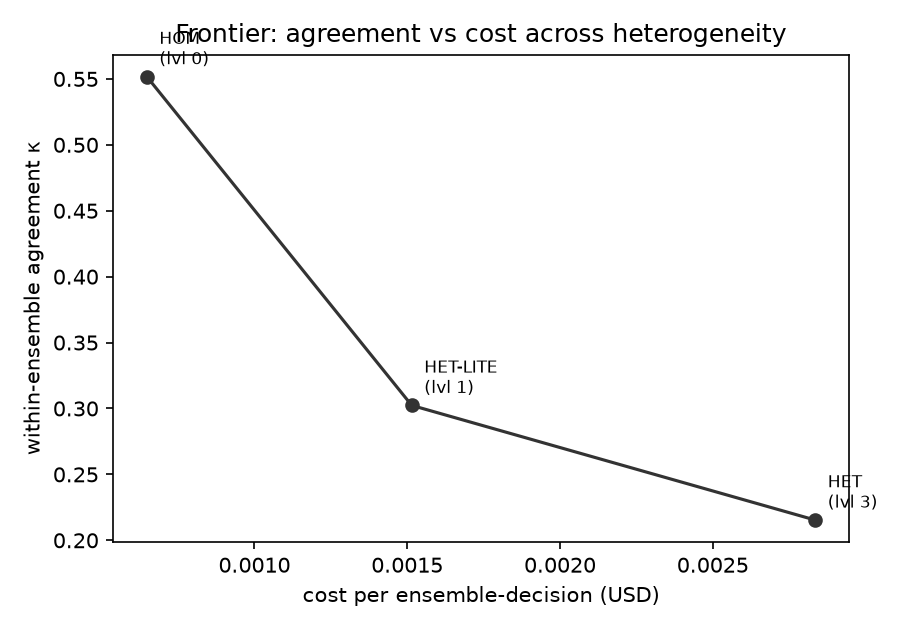
\includegraphics[width=\columnwidth]{fig1_frontier.png}
\caption{Agreement--cost frontier. Within-ensemble Fleiss' $\kappa$ ($y$) versus
cost per ensemble decision ($x$) at heterogeneity levels $\{0, 1, 3\}$. Lower
$\kappa$ $=$ more independent agents; the horizontal spread is the cost
premium.}
\label{fig:frontier}
\end{figure}

\subsection{Measurement protocol: sampling non-determinism inflates $\kappa$}
\label{sec:protocol}
\paragraph{Exactly what was shared}
In our first (pilot) implementation the random seed was derived per ensemble
\emph{run} rather than per agent: every one of the five same-model agents in a
cell received the identical seed, and therefore the identical sampling
trajectory, from the provider's decoder. With temperature sampling made
deterministic by a shared seed, five ``independent'' gpt-5.4-nano calls on the
same prompt returned near-verbatim outputs, driving $\kappa_{\mathrm{HOM}}$
artificially toward 1. The fix is one line of seed derivation: give each agent a
unique, reproducible seed keyed by its position (Fig.~\ref{fig:seed}), so the
five agents draw independent samples from the same model. We stress that this is
the only change; the prompt, model, temperature, and grid are identical before
and after.

\begin{figure}[!t]
\centering
\begin{lstlisting}
# Before (artifact): one seed shared by all agents in a run
seed = f(master, run)
for agent in 1..5:
    call(model, prompt, seed)  # identical draw

# After (fix): unique per-agent seed, independent draws
seed = SHA256(master, run, config,
              ticker, date, agent) & 0x7FFFFFFF
call(model, prompt, seed)  # independent draw per agent
\end{lstlisting}
\caption{The one-line fix. The pilot derived the seed per run, so all five
same-model agents shared a sampling path; the study derives a distinct
integer-safe seed per agent, restoring independent draws from the same model.}
\label{fig:seed}
\end{figure}

\paragraph{Ruling out adjacent explanations}
A reader may wonder whether the near-duplicate pilot outputs came instead from
response caching or request batching. Neither applies: provider- and client-side
prompt caching was disabled (no cache headers; each call is a fresh completion),
and every agent call is an independent HTTP request---agents are never batched
into a single multi-sample call. The duplication was attributable solely to the
shared seed, which the fix removes.

Our within-run vs.\ cross-run diagnostic (Table~\ref{tab:nondet}) verifies the
fix rather than merely asserting it: after adopting per-agent independent draws,
the HOM within$-$cross gap is $0.0006\approx 0$, confirming the homogeneous
agents are genuinely independent rather than copies (a residual gap near 1 would
have signalled surviving duplication). In a controlled pilot, the artifact was
severe: the same primary effect measured $\Delta\kappa=0.485$ under a shared
sampling context but $0.113$ under independent draws---a $\sim$4$\times$
over-statement produced entirely by the measurement apparatus
(Fig.~\ref{fig:trap}). We recommend the independent-draw protocol and the
within/cross diagnostic as a standard check for any LLM-ensemble agreement
study.

The negative within$-$cross gaps for the heterogeneous configurations
($-0.048$ and $-0.074$; Table~\ref{tab:nondet}) are expected and benign, and act
as a further consistency check. Pooling the three runs' draws into a single
cross-run $\kappa$ re-introduces same-model replicate agreement---a model's
repeated draws for a cell tend to be mutually similar---which raises the pooled
$\kappa$ above the single-draw within-run value; the more diverse the ensemble,
the larger this pooling effect, hence the monotonic ordering of the gaps ($0$ for
HOM, $-0.048$ for HET-LITE, $-0.074$ for HET). Crucially, our primary endpoint
uses the conservative within-run (single-draw) estimate, so this pooling cannot
inflate $\Delta\kappa$; the direction of the gaps merely reconfirms that
additional same-model draws add correlation.

\begin{table}[!t]
\centering
\caption{Non-determinism check: within-run vs.\ cross-run $\kappa$ (must be
$\approx 0$ for the primary/homogeneous configuration).}
\label{tab:nondet}
\begin{tabular}{lccc}
\toprule
Config & within & cross & within$-$cross \\
\midrule
HOM & 0.552 & 0.551 & $+0.001$ \\
HET-LITE & 0.302 & 0.350 & $-0.048$ \\
HET & 0.215 & 0.289 & $-0.074$ \\
\bottomrule
\end{tabular}
\end{table}

\begin{figure}[!t]
\centering
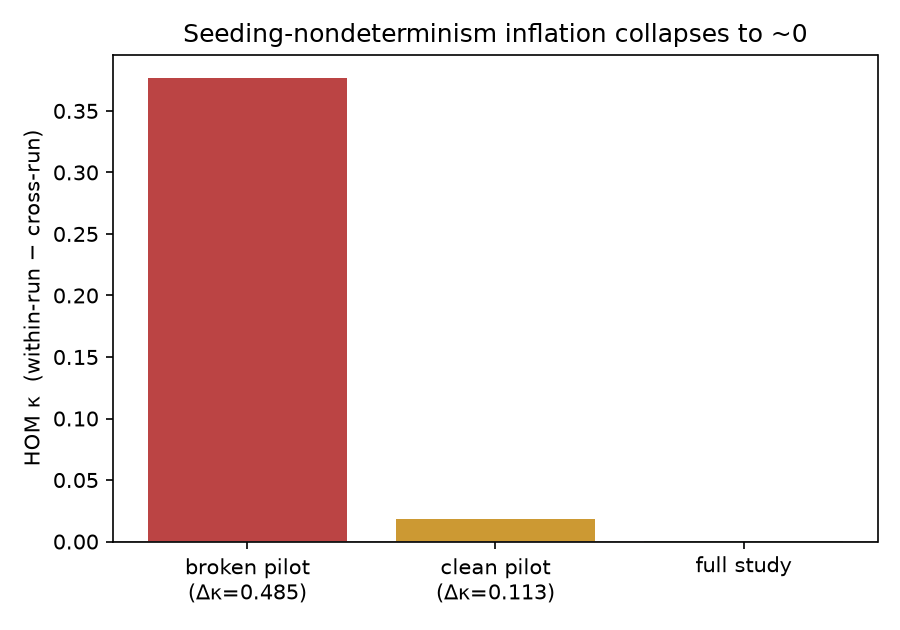
\includegraphics[width=\columnwidth]{fig2_protocol.png}
\caption{The measurement trap. Homogeneous within$-$cross $\kappa$ gap
collapses from a seed-shared pilot ($\Delta\kappa=0.485$) to the
independent-draw pilot ($\Delta\kappa=0.113$) to $\approx 0$ in the full study,
showing that shared-context sampling non-determinism, not model similarity,
produced the inflation.}
\label{fig:trap}
\end{figure}

\subsection{Provider-pair agreement}
The pairwise direction-agreement matrix (Fig.~\ref{fig:provider}) shows agents
from the same provider agree far more than cross-provider pairs: within-provider
agreement is $0.92$ (Google) and $0.80$ (OpenAI), whereas cross-provider pairs
range $0.43$--$0.63$. This is the mechanism behind the frontier: provider
identity, not merely stochasticity, is the dominant axis of agent
(dis)agreement.

\begin{figure}[!t]
\centering
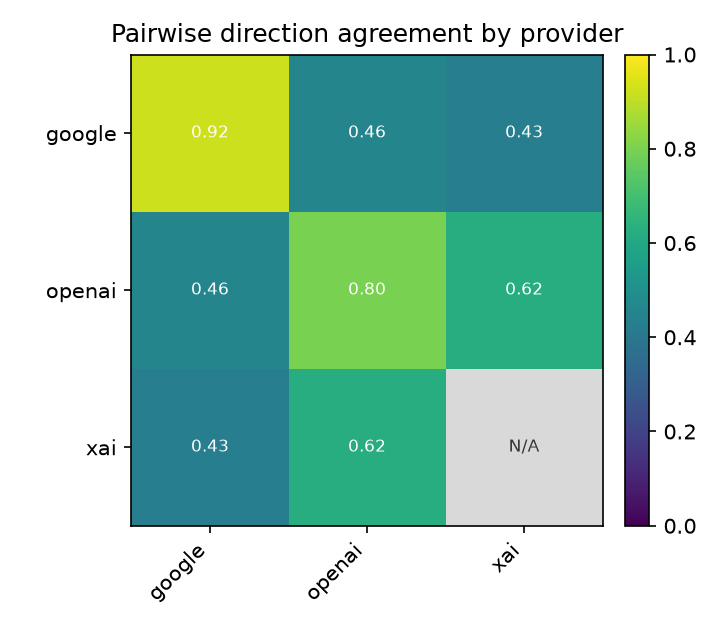
\includegraphics[width=0.85\columnwidth]{fig3_provider_heatmap.png}
\caption{Pairwise directional-agreement matrix by provider. Diagonal
(within-provider) agreement greatly exceeds off-diagonal (cross-provider), the
source of ensemble de-correlation. The xAI--xAI diagonal is undefined (marked
N/A, not 0): each HET cell contains a single xAI agent, so no within-xAI agent
pair exists.}
\label{fig:provider}
\end{figure}

\subsection{Accuracy proxy (secondary; honest null)}
As a pre-declared secondary, descriptive axis, we score each ensemble's
majority-vote direction against the sign of the realized 20 trading-day forward
return (HOLD abstains). Directional hit-rates are $0.438$ (HOM), $0.463$
(HET-LITE), and $0.488$ (HET), with overlapping 95\% Wilson intervals
(Table~\ref{tab:acc}). The study is powered for $\kappa$, not for accuracy; we
therefore draw no conclusion that heterogeneity improves accuracy. The slight
upward trend is reported for completeness only.

\begin{table}[!t]
\centering
\caption{Accuracy proxy (SECONDARY; underpowered by design). Hit-rate of
majority-vote direction vs.\ 20-day forward-return sign; HOLD abstains.}
\label{tab:acc}
\begin{tabular}{lccc}
\toprule
Config & hit-rate & $n$ & 95\% CI (Wilson) \\
\midrule
HOM & 0.438 & 315 & $[0.384,\ 0.493]$ \\
HET-LITE & 0.463 & 339 & $[0.411,\ 0.516]$ \\
HET & 0.488 & 525 & $[0.445,\ 0.530]$ \\
\bottomrule
\end{tabular}
\end{table}

\subsection{Beyond average accuracy: manufactured consensus and tail risk
(exploratory)}
Average directional accuracy is flat (Sec.~5.6), but average
accuracy is not the only quantity a practitioner cares about: in a decision
setting, a committee that is confidently and unanimously wrong is more dangerous
than one whose members hedge. We therefore examine, post hoc and exploratorily
(no pre-registered hypothesis; no confidence intervals promoted to our headline
claims), how heterogeneity reshapes the structure of consensus rather than its
mean correctness. All quantities below are computed on the same frozen grid,
scoring each five-agent ensemble decision against the realized forward-return
sign (Table~\ref{tab:consensus}).

Three patterns emerge: two strictly monotone in heterogeneity, while the
third---confident collective error---saturates from the first heterogeneous
agent onward. (i)~\emph{Unanimity.} The rate at which all five agents return one
identical direction falls from $0.591$ (HOM) to $0.315$ (HET-LITE) to $0.267$
(HET): homogeneous committees manufacture consensus more than twice as often.
(ii)~\emph{Confident collective error.} The rate of decisions that are
unanimous, directional, and wrong---the exact ``manufactured-consensus'' failure
that monoculture warnings describe~\cite{kim2025correlated}---is $0.058$ for HOM
versus $0.032$ for HET, so the homogeneous ensemble commits confident collective
blunders at $1.84\times$ the fully heterogeneous rate. Notably, HET-LITE already
achieves essentially the full reduction ($0.030$ vs.\ $0.032$ for HET) at a
$\sim$2.3$\times$ rather than $\sim$4.4$\times$ premium: in this setting, a
single second-provider agent captures nearly all of the tail-risk benefit,
making HET-LITE the efficient operating point on the frontier.
(iii)~\emph{Error pile-on.} Conditional on the majority vote being wrong, the
fraction of agents that nonetheless endorse the wrong call is $0.824$ (HOM),
$0.761$ (HET-LITE), $0.636$ (HET): when a heterogeneous ensemble errs, its
members are far more likely to have dissented, leaving a usable disagreement
signal that a homogeneous ensemble erases. Read together, these indicate that
the priced de-correlation buys a measurable reduction in \emph{tail risk}---fewer
confident collective errors---even where it buys no gain in mean accuracy, which
for a finance application is arguably the more relevant benefit.

We caution against over-reading conviction as calibrated confidence: per-agent
directional hit-rate is essentially flat across self-reported conviction buckets
and never exceeds chance by a reliable margin in any configuration
(Fig.~\ref{fig:cal}), consistent with the accuracy null. Heterogeneity's benefit
here is in the structure of collective agreement, not in per-call calibration.
These exploratory results motivate, but do not establish, a downstream
advantage; we frame them as hypotheses for a confirmatory, appropriately powered
follow-up.

\begin{table}[!t]
\centering
\caption{Consensus structure by heterogeneity (exploratory; 3{,}600 scoreable
five-agent decisions per config). ``Unan.\ wrong'' $=$ all five agents agree on
one directional call that is wrong; ``pile-on'' $=$
$P(\mathrm{agent\ endorses\ majority}\mid\mathrm{majority\ wrong})$.}
\label{tab:consensus}
\begin{tabular}{lccc}
\toprule
Config & unanimity & unan.\ wrong & pile-on \\
\midrule
HOM & 0.591 & 0.058 & 0.824 \\
HET-LITE & 0.315 & 0.030 & 0.761 \\
HET & 0.267 & 0.032 & 0.636 \\
\bottomrule
\end{tabular}
\end{table}

\begin{figure}[!t]
\centering
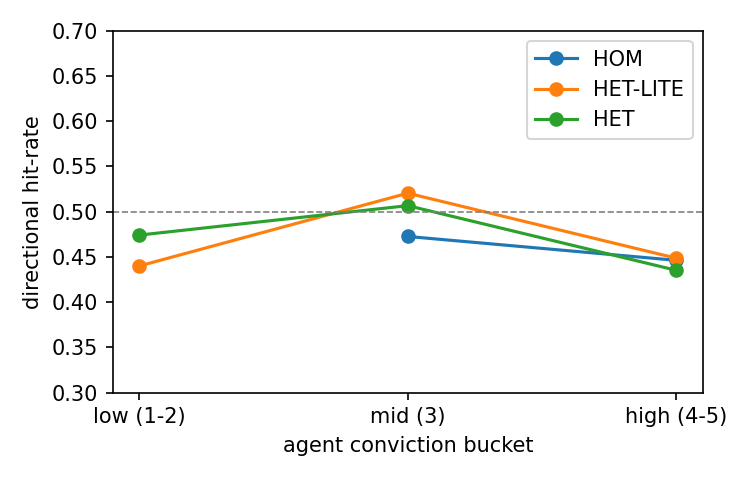
\includegraphics[width=\columnwidth]{fig5_calibration.png}
\caption{Conviction is not calibrated. Per-agent directional hit-rate by
self-reported conviction bucket; no configuration rises reliably above chance
($0.5$, dashed) and higher conviction does not imply higher accuracy, consistent
with the accuracy null.}
\label{fig:cal}
\end{figure}

\subsection{Robustness: capability-matched control}
To separate provider diversity from capability tier---the study's principal
confound---we ran a pre-registered control that holds capability approximately
constant while varying provider: Het-SameTier, comprising three gpt-5.4-nano and
two gemini-3.1-flash-lite agents, i.e.\ the efficient tier of each provider (no
efficient-tier xAI model is exposed, so the control is OpenAI vs.\ Google).
Compared against the identical HOM baseline over the same $100\times 12$ grid
(36{,}000 calls), the control yields $\kappa_{\mathrm{HOM}}=0.552$ and
$\kappa_{\mathrm{HET\text{-}SameTier}}=0.236$, a contrast of
\[
\Delta\kappa_{\mathrm{HOM-SameTier}}=0.315,\quad
95\%\ \mathrm{CI}\ [0.288,\ 0.341],
\]
which excludes zero. This capability-matched effect recovers $\approx$94\% of
the full flagship-mixture effect ($0.336$), demonstrating that the de-correlation
is driven overwhelmingly by provider identity rather than capability tier. The
capability confound is therefore not a plausible explanation for the primary
result. (The reproduction of $\kappa_{\mathrm{HOM}}=0.552$ to four decimals
across two independently collected datasets also re-confirms determinism of the
homogeneous baseline.)

\subsection{Robustness: temperature sensitivity}
Agreement is mechanically a function of sampling temperature, so a natural
concern is that our primary effect is an artifact of the single operating point
$T=0.7$. We therefore re-ran a small stratified subgrid (8 equities $\times$ 2
dates $\times$ 3 configs $\times$ 3 runs, written to separate files that never
touch the frozen study) at $T\in\{0.0,0.7,1.0\}$ and recomputed $\kappa$ and
the primary contrast at each temperature (Table~\ref{tab:temp}). Two things are
stable and one is not. Stable: the ordering
$\kappa_{\mathrm{HOM}}>\kappa_{\mathrm{HET\text{-}LITE}}>\kappa_{\mathrm{HET}}$
holds at every temperature, and the primary contrast
$\Delta\kappa(\mathrm{HOM}-\mathrm{HET})$ is positive with a 95\% CI excluding
zero at every temperature ($0.299$, $0.509$, $0.385$ at $T=0.0,0.7,1.0$). Not
stable: the absolute $\kappa$ levels vary non-monotonically with $T$ (e.g.\
$\kappa_{\mathrm{HOM}}$ ranges $0.33$--$0.67$), because temperature shifts both
within-cell concordance and the directional marginals (at $T=0$ the homogeneous
marginal is near-uniform across BUY/HOLD/SELL, lowering chance-corrected
agreement despite greedy decoding; at $T=0.7$--$1.0$ it concentrates on HOLD).
The takeaway is that our conclusion is a statement about the contrast between
configurations, which is temperature-robust, not about any absolute agreement
level, which is not. This subgrid is a documented pre-registration amendment and
is analyzed by the same seeded estimator as the main study.

\begin{table}[!t]
\centering
\caption{Temperature-sensitivity robustness ($8\times 2$ subgrid, 3 runs per
cell). The ordering ($\kappa_{\mathrm{HOM}}>\kappa_{\mathrm{HET\text{-}LITE}}>\kappa_{\mathrm{HET}}$)
and the primary contrast $\Delta\kappa_{\mathrm{HOM-HET}}$ (positive, CI excludes
0) hold at every temperature; absolute $\kappa$ levels vary non-monotonically, so
it is the contrast, not the absolute agreement, that is temperature-stable.}
\label{tab:temp}
\begin{tabular}{lcccc}
\toprule
$T$ & $\kappa_{\mathrm{HOM}}$ & $\kappa_{\mathrm{HET\text{-}LITE}}$ &
$\kappa_{\mathrm{HET}}$ & $\Delta\kappa$ [95\% CI] \\
\midrule
0.0 & 0.33 & 0.17 & 0.03 & 0.30 $[0.16,\ 0.44]$ \\
0.7 & 0.67 & 0.38 & 0.16 & 0.51 $[0.21,\ 0.78]$ \\
1.0 & 0.53 & 0.27 & 0.15 & 0.38 $[0.19,\ 0.54]$ \\
\bottomrule
\end{tabular}
\end{table}

\section{Discussion}
Our central result gives quantitative teeth to an intuition: a homogeneous LLM
committee is substantially an echo chamber ($\kappa=0.55$), and cross-provider
heterogeneity is what actually makes its members think independently
($\kappa=0.22$), for a well-characterized $\sim$4.4$\times$ cost. The
provider-pair matrix shows this de-correlation is driven by provider identity
rather than sampling noise. Crucially, de-correlation is a necessary but not
sufficient condition for ensemble benefit: independence only helps if the
independent opinions are also informative. Our honest null on average accuracy,
read alongside the correlated-error / monoculture findings of Kim \textit{et
al.}~\cite{kim2025correlated}, cautions that buying disagreement does not
automatically buy correctness. Yet our exploratory analysis of consensus
structure (Sec.~5.7) suggests the premium is not valueless in this setting:
homogeneous committees produce confident, unanimous, wrong calls at $1.84\times$
the heterogeneous rate, so the independence appears to buy tail-risk reduction
even without a mean-accuracy gain---a hypothesis we flag for confirmatory
follow-up. For practitioners, the frontier is directly actionable: teams paying
the heterogeneity premium should verify that the additional independence
translates into a downstream objective (calibration, robustness, or reduced
collective-error rate) for their task rather than assuming it. Our own data
already hint at where the value concentrates: because the confident-collective-
error rate saturates from the first heterogeneous agent onward, HET-LITE
captures nearly all of the tail-risk benefit at a $\sim$2.3$\times$ rather than
$\sim$4.4$\times$ premium, making a single second-provider agent the efficient
operating point in this setting.

Methodologically, the sampling-non-determinism trap (Section~\ref{sec:protocol})
is, we argue, of independent value: any study that measures LLM-ensemble
agreement without controlling the sampling context risks a multiplicative
over-statement.

\section{Threats to Validity}
\textbf{Heterogeneity vs.\ capability confound.}
HOM uses five instances of a small efficient model, whereas heterogeneous
configurations add larger, different-provider models; part of the measured
de-correlation could in principle reflect capability differences rather than
provider identity per se. Two pieces of evidence bound this concern. First, the
provider-pair analysis (Fig.~\ref{fig:provider}) is a within-cell comparison: for
a fixed cell, all agents receive the identical prompt, yet same-source agent
pairs agree far more ($0.80$--$0.92$) than cross-source pairs ($0.43$--$0.63$),
indicating that source identity---not merely stochasticity or prompt
difficulty---drives disagreement. Second, the effect is monotone and significant
at every increment of heterogeneity (Table~\ref{tab:endpoints}), including the
HET-LITE$\to$HET step, which adds provider diversity without a systematic
capability jump. Third and most directly, our capability-matched control
(Section~5.8) holds tier approximately constant and still yields
$\Delta\kappa=0.315$ (95\% CI $[0.288, 0.341]$), $\approx$94\% of the full
effect, so the de-correlation is provider-driven rather than tier-driven. The
residual limitation is scope: the control contrasts two providers (OpenAI vs.\
Google), since no efficient-tier xAI model is currently exposed; a fully
tier-matched three-provider control awaits such a model.

\textbf{Single task domain.}
All results are for one directional financial-analysis task with a single prompt
template; richer analyst tasks may exhibit different agreement structure, and we
make no claim about LLM ensembles in general. Two factors bound this concern.
First, the driving mechanism---higher within-provider than cross-provider
agreement (Fig.~\ref{fig:provider})---is a property of the models, not of the
finance framing, so we expect the ordering (though not the magnitude) to
transfer. Second, we pre-register an out-of-domain replication as immediate
future work: the identical pipeline (three configs, per-agent seeding,
per-run-averaged $\kappa$) applied to a three-class classification task (e.g.\
sentiment) on a small grid, reported without new confidence claims, to test
whether the HOM $>$ HET-LITE $>$ HET ordering is finance-specific. Finance is
arguably a hard case for stability, given the regime shifts spanned by our
dates, which makes the monotone de-correlation we observe a conservative
demonstration.

\textbf{Model-version pinning.}
Providers update models; we mitigate by pinning exact strings and treating the
hash-frozen dataset as the object of record.

\textbf{Single-run collection.}
Confirmatory data are collected once; provider-side drift within the window is
not averaged out.

\textbf{Accuracy underpowered.}
The design is powered for $\kappa$, not accuracy; the accuracy proxy is
descriptive with wide intervals and must not be read as an alpha claim.

\textbf{Generalization.}
Findings pertain to these three ensemble recipes, five agents, and this provider
set; other sizes, tasks, and mixes may differ.

\section{Conclusion}
We present a pre-registered, 54{,}000-call measurement of how cross-provider
heterogeneity de-correlates LLM ensembles and what it costs. Heterogeneity
reduces within-ensemble agreement monotonically---$\Delta\kappa=0.336$ (95\% CI
$[0.304, 0.369]$)---at a $\sim$4.4$\times$ inference-cost premium, defining an
explicit agreement--cost frontier. We contribute a measurement protocol that
removes a $\sim$4$\times$ inflation from shared-context sampling
non-determinism, and we release a frozen, reproducible artifact. We find no
reliable average-accuracy benefit at this scale, situating the result within the
algorithmic-monoculture literature: diversity buys disagreement, but disagreement
must still be shown to buy value. An exploratory analysis nonetheless indicates
one concrete value---homogeneous ensembles commit confident, unanimous,
directional errors at $1.84\times$ the heterogeneous rate---suggesting tail-risk
reduction that a confirmatory study should test. A pre-registered,
capability-matched control establishes that the effect is provider-driven rather
than a capability-tier artifact ($\Delta\kappa=0.315$, 95\% CI $[0.288, 0.341]$);
the remaining methodological gap is a fully tier-matched three-provider control,
which awaits an efficient-tier model from a third provider. Two further steps
follow: an out-of-domain replication to test whether the de-correlation ordering
is task-general, and connecting the priced independence to downstream objectives
(calibration, robustness, collective-error rate) so that it can be shown to buy
value in this and other settings.

\section*{Data and Code Availability}
To support reproduction, we release: (i)~the immutable, read-only,
SHA-256-stamped raw dataset (\texttt{runs.csv}; 54{,}000 logged calls with
per-call model, seed, prompt hash, timestamp, tokens, cost, and raw response);
(ii)~the pre-registration and the cryptographic freeze receipt; (iii)~the
deterministic, seeded analysis pipeline that regenerates every figure and table
in this paper byte-for-byte, together with a replication check; and (iv)~the
orchestration harness including the Het-SameTier control configuration. Artifacts
are archived at [Zenodo / Code Ocean DOI, to be minted on acceptance] and
mirrored at
\url{https://github.com/samirrc2/price-of-decorrelation}.
The dataset SHA-256 and commit hash are recorded in the manuscript's
supplementary manifest.

\section*{Acknowledgment}
The authors thank colleagues and reviewers for feedback.

\bibliographystyle{IEEEtran}
\bibliography{references}

\begin{IEEEbiographynophoto}{Samir Chincholikar}
Independent researcher. Research interests include large language models,
multi-agent systems, machine learning evaluation, and reproducible empirical
methods.
\end{IEEEbiographynophoto}

\begin{IEEEbiographynophoto}{Robin Chawla}
Independent researcher. Research interests include large language models,
systems, and reproducible computational science.
\end{IEEEbiographynophoto}

\end{document}
